\documentclass[[12pt,twoside]{book}
\usepackage{_my_document_style}
\begin{document}
%
\begin{figure}[t]%[H]%[!htbp]
  %\centering
  %\checkoddpage
  %\centering
    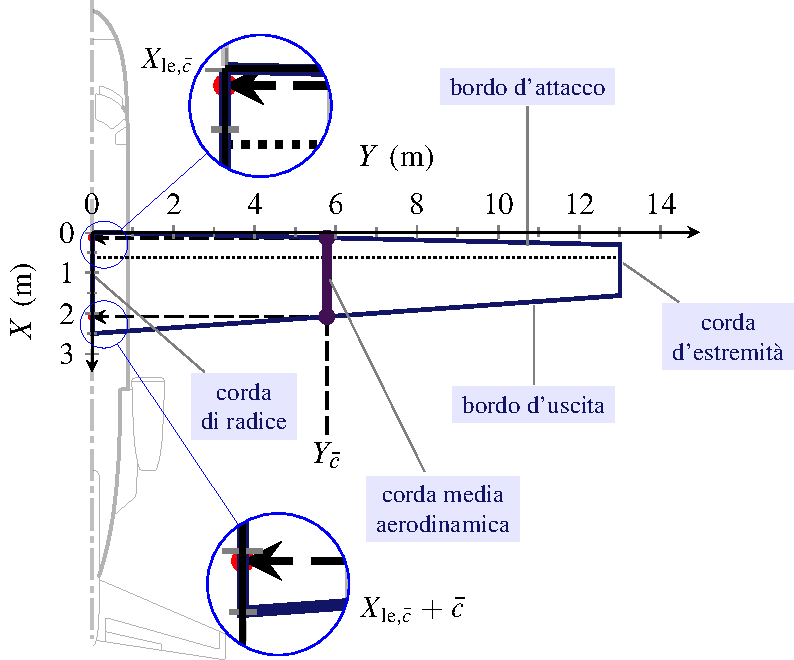
\includegraphics[width=0.78\textwidth]{Chapter_2/geometric_characteristics_of_a_straight_and_tapered_wing/wing_planform_basic_0A_drawing.pdf}%
  \caption{\finalhyphendemerits=1000
            Planform of the wing assigned in the example~\ref{example:Geometric:Characteristics:Of:A:Straight:And:Tapered:Wing}.}
  \label{fig:Wing:Planform:Basic:Drawing:AB}%
\end{figure}%
%
\def\mySpanWingMT{26.000000}
\def\myChordRootWingMT{2.500000}
\def\myChordTipWingMT{1.250000}
\def\myTaperRatioWing{0.500000}
\def\myAreaWingMTsquared{48.750000}
\def\myMACWingMT{1.944444}
\def\myYMACWingMT{5.777778}
\def\myXLEMACWingMT{0.138889}
\def\myLambdaCQuarterDeg{0.000000}
\def\myLambdaLEDeg{1.377037}
\def\myLambdaLERad{0.024034}
\def\myAspectRatioWing{13.866667}
\def\myCoefficientA{-0.096154}
\def\myCoefficientB{2.500000}

%
\begin{myExampleX}{Geometric characteristics of a straight and tapered wing}{\ding{46}}% \ \Keyboard\ %
\label{example:Geometric:Characteristics:Of:A:Straight:And:Tapered:Wing}
%

Let us consider a wing with a finite wingspan equal to $b=\SI[round-precision=1]{\mySpanWingMT}{\metre}$,
straight leading and trailing edges and null sweep angle that is: $\Lambda_{c/4}=\SI[round-precision=0]{\myLambdaCQuarterDeg}{\degree}$.
Unlike the previous example, the wing assigned here is tapered, i.e.
the chord of the different wing sections varies linearly with distance $Y$ from the center plane. The root chord is
$c_\mathrm{r}=\SI[round-precision=2]{\myChordRootWingMT}{\metre}$ and the tip chord is $c_\mathrm{t}=\SI[round-precision=2]{\myChordTipWingMT}{\metre}$.
We want to calculate the following quantities:

\adjustbox{center=\textwidth}{%
$S$\,, $\AR$\,, $\Lambda_\mathrm{le}$\,, $\bar{c}$\,, $X_{\mathrm{le},\bar{c}}$\,, $Y_{\bar{c}}$
}% \,, $Y_{\bar{c}}$
\medskip

Given the two root and tip chords, the taper ratio must be evaluated as:
\[
\lambda
  =\frac{c_\mathrm{t}}{c_\mathrm{r}}
  =\frac{\SI[round-precision=2]{\myChordTipWingMT}{\metre}}{\SI[round-precision=2]{\myChordRootWingMT}{\metre}}
  = \SI[round-precision=2]{\myTaperRatioWing}{} 
\]
As for the law of the chords , we obtain:
$c ( Y ) = A_c \, Y + B_c$. By imposing that $c(0)=c_\mathrm{r}$ and $c(\frac{1}{2}b)=c_\mathrm{t}$,
we can calculate the coefficients of the linear law:
\[
A_c
  = \frac{c_\mathrm{t} - c_\mathrm{r}}{b/2}
  = 
    2 \frac{
      \SI[round-precision=2]{\myChordTipWingMT}{\metre} - \SI[round-precision=2]{\myChordRootWingMT}{\metre}
    }{
      \SI[round-precision=2]{\mySpanWingMT}{\metre}
    }
  =  \SI[round-precision=3]{\myCoefficientA}{} 
\]
\[
B_c
  = c_\mathrm{r}
  =  \SI[round-precision=2]{\myCoefficientB}{\metre} 
\]
therefore
\[
c \big( Y \big) = A_c \, Y + B_c
  = \SI[round-precision=3]{\myCoefficientA}{} \, Y
    + \SI[round-precision=2]{\myCoefficientB}{\metre}
\]
The wing surface in this case is nothing more than the area of two trapezoids,
each of a major base $c_\mathrm{r}$, minor base $c_\mathrm{t}$ and height $\frac{1}{2}b$, and is calculated as follows:
\[
\begin{split}
S & {}= \frac{b}{2} \, c_\mathrm{r} \, \big( 1 + \lambda \big) \\
  & {}=
    \num{0.5} \cdot \SI[round-precision=1]{\mySpanWingMT}{\metre}
      \cdot \SI[round-precision=2]{\myChordRootWingMT}{\metre}
      \cdot \big( 1 + \SI[round-precision=2]{\myTaperRatioWing}{} \big) 
    =  \SI[round-precision=1]{\myAreaWingMTsquared}{\metre^2} 
\end{split}
\]
It is easy to verify that you get the same result if you apply the calculation formula.
\[
\begin{split}
S & {}= 2\, \int_0^{b/2} c(Y) \diff{Y} = 2\, \int_0^{b/2} \Big( A_c Y + B_c \Big) \diff{Y}
\\
  & {}= 2\, 
    \int_{\SI{0}{m}}^{\calcSI[round-precision=1,fixed-exponent=0,scientific-notation=fixed]{0.5*\mySpanWingMT}{\metre}}
    \Big( 
      \SI[round-precision=3]{\myCoefficientA}{} \, Y
      + \SI[round-precision=2]{\myCoefficientB}{\metre}
    \Big) \diff{Y}
    = 2\, \bigg[
      \SI[round-precision=3]{\myCoefficientA}{} \, \dfrac{Y^2}{2}
      + \SI[round-precision=2]{\myCoefficientB}{\metre} \, Y
    \bigg]_{\SI{0}{m}}^{\calcSI[round-precision=1,fixed-exponent=0,scientific-notation=fixed]{0.5*\mySpanWingMT}{\metre}}
\\
  & {}= 2\,
    \Big(
      \SI[round-precision=3]{\myCoefficientA}{}
        \cdot 
        \calcSI[round-precision=1,fixed-exponent=0,scientific-notation=fixed]{
          0.5*\mySpanWingMT*0.5*\mySpanWingMT*0.5
        }{\metre^2}
        + 
        \calcSI[round-precision=1,fixed-exponent=0,scientific-notation=fixed]{
          \myCoefficientB * 0.5*\mySpanWingMT
        }{\metre^2}
    \Big) - \SI{0}{\metre^2}
\end{split}
\]
At this point we can calculate the wing aspect ratio, that is:
\[
\AR
  = \frac{b^2}{S}
  = \frac{\big(\SI[round-precision=1]{\mySpanWingMT}{m}\big)^2}{\SI[round-precision=1]{\myAreaWingMTsquared}{m^2}}
  =   \num[round-precision=2]{\myAspectRatioWing} 
\]
It is known that the line joining the points along the individual chords $c(Y)$ distant $c(Y)/n$ from the local leading edge forms a sweep angle $\Lambda_{c/n}$ connected to that of the leading edge $\Lambda_\mathrm{le}$ from the following relationship:
\[
\tan\Lambda_{c/n} = \tan\Lambda_\mathrm{le}-\dfrac{(4/n)(1-\lambda)}{\AR(1+\lambda)}
\]
From this, for a sweep angle
$\Lambda_\mathrm{c/4}=\SI[round-precision=1]{\myLambdaCQuarterDeg}{\degree}$
of the line of the quarter chords, we obtain:
\[
\tan
\SI[round-precision=0]{\myLambdaCQuarterDeg}{}
   = \tan\Lambda_\mathrm{le} 
      - \dfrac{
         \num[round-precision=2]{1.0}
         \cdot (1-\SI[round-precision=2]{\myTaperRatioWing}{})
      }{
         \num[round-precision=2]{\myAspectRatioWing}
         \cdot (1+\SI[round-precision=2]{\myTaperRatioWing}{})} 
   \quad
   \Rightarrow
   \quad
   \Lambda_\mathrm{le}
      =  \SI[round-precision=4]{\myLambdaLERad}{\radian} 
      =  \SI[round-precision=1]{\myLambdaLEDeg}{\deg} 
\]
The mean aerodynamic chord in this case is:
\[
\begin{split}
\bar{c} & {}= \frac{2}{3} \, c_\mathrm{r} \, \frac{1+\lambda + \lambda^2}{1+\lambda} \\
  & {}=
    \num{0.667} \cdot \SI[round-precision=2]{\myChordRootWingMT}{\metre}
      \cdot 
        \frac{
          1 + \SI[round-precision=2]{\myTaperRatioWing}{} + \SI[round-precision=2]{\myTaperRatioWing}{}^2
        }{
          1 + \SI[round-precision=2]{\myTaperRatioWing}{}
        }
    =  \SI[round-precision=2]{\myMACWingMT}{\metre} 
\end{split}
\]
that is, an intermediate value between that of the root chord (\SI[round-precision=2]{\myChordRootWingMT}{\metre}) 
and that of the tip chord (\SI[round-precision=2]{\myChordTipWingMT}{\metre}),
closer to the former than to the latter.
The longitudinal distance of the leading edge of the aerodynamic middle chord from the leading edge of the root chord is :
\[
\begin{split}
X_{\mathrm{le},\bar{c}} 
  & {}=
    \frac{b}{6} \, \frac{1+2\lambda}{1+\lambda} \tan\Lambda_\mathrm{le} \\[3pt]
  & {}=
    \frac{\SI[round-precision=1]{\mySpanWingMT}{\metre}}{6}
      \cdot 
      \frac{
        1 + 2\cdot\SI[round-precision=2]{\myTaperRatioWing}{}
      }{
        1 + \SI[round-precision=2]{\myTaperRatioWing}{}
      }
      \cdot \tan \big( \SI[round-precision=3]{\myLambdaLERad}{\radian} \big)
    =  \SI[round-precision=2]{\myXLEMACWingMT}{\metre} % \myXMACLEToWingRootLEMT
\end{split}
\]
It is observed that the tapered wing, even if with zero sweep angle, corresponds to a $X_{\mathrm{le},\bar{c}}$ not null. This means that the projection of the wing section having chord equal to $\bar{c}$ in the middle plane it is further back than the root chord. Moreover,given the value of $\bar{c}$ previously calculated, this projection is internal to the root chord, that is:
$X_{\mathrm{le},\bar{c}}+\bar{c}<c_\mathrm{r}$.
The  station $Y_{\bar{c}}$ to which the law of the chords $c(Y)$ assumes value $\bar{c}$ is
\[
\begin{split}
Y_{\bar{c}} 
  & {}=
    \frac{b}{6} \, \frac{1+2\lambda}{1+\lambda} = \\[3pt]
  & {}=
    \frac{\SI[round-precision=1]{\mySpanWingMT}{\metre}}{6}
      \cdot 
      \frac{
        1 + 2\cdot\SI[round-precision=2]{\myTaperRatioWing}{}
      }{
        1 + \SI[round-precision=2]{\myTaperRatioWing}{}
      }
    =  \SI[round-precision=2]{\myYMACWingMT}{\metre} 
\end{split}
\]
The calculated value corresponds to a station along the wingspan closest to the root the to the tip.
\end{myExampleX}
\end{document} 
